\section{Implementation}
\label{sec:implementation}

\subsection{Overview}
%To meet the performance requirements of the data center, we implemented \OurSys
We implemented \OurSys
on the Xilinx Zynq UltraScale+ MPSoC ZCU102 Evaluation Kit.  This board has 4 SFP+ cages, and we process network traffic on its
ZU9EG System-on-Chip FPGA, which consists of a quad-core ARM Cortex-A53, a
dual-core ARM Cortex-R5, and a programmable fabric with 274K lookup tables
(LUTs) and 1800 18Kb embedded memories (BRAMs).

\begin{figure}
  \centering
  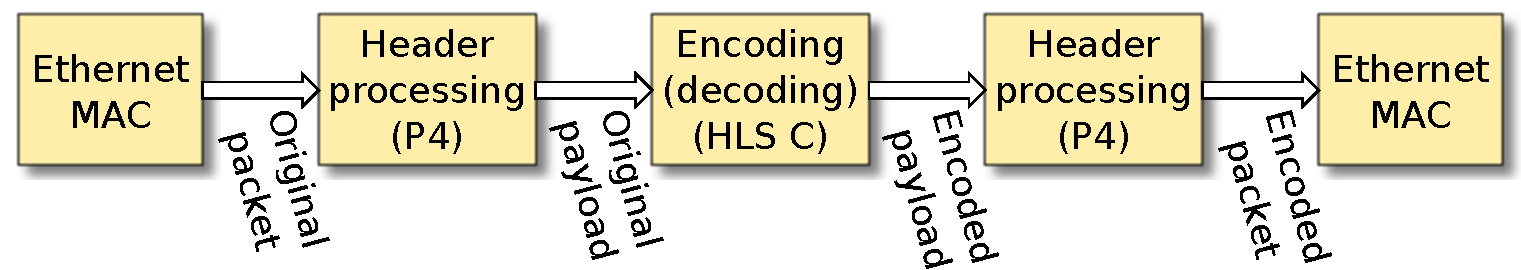
\includegraphics[width=0.4\paperwidth]{Top_level.pdf}
  \caption{\label{fig:toplevel} Block diagram of FEC encoder / decoder pipeline.
  }
\end{figure}

A top-level diagram of the implementation is shown in Fig.~\ref{fig:toplevel}.
%Packets arrive on one of the 4 SFP+ cages via a 10Gbps Ethernet cable.
%A dedicated 10~Gigabit Transceiver deserializes the packets.  After further
%processing by a dedicated Ethernet PHY and in-fabric MAC layer, the entire
%packet including Ethernet header is output on a 64-bit AXI Stream bus at 160\,MHz.
%
%The next stage in the pipeline performs packet header preprocessing.  With
%ease of implementation and portability in mind, we implemented this in P4, a
%domain-specific programming language for packet processing that is target- and
%protocol-agnostic \cite{p4_sigcomm_review2014}.
We implement header processing in
P4~\cite{Bosshart:2014:PPP:2656877.2656890}, which is compiled to FPGA
logic using Xilinx's SDNet tool suite.  Header processing (described
further in~\S\ref{sec:impl:header-processing}) includes the frame
tagging described in~\S\ref{sec:design}.

The frame is then forwarded to the FEC core, which can be an encoder (for the Sending Proxy) or decoder (for the
Receiving Proxy).
%In both cases, the FEC core
%produces payloads that are the result of, respectively, encoding or decoding
%the received group of payloads.  Similar to the header processing, the FEC core
%was also created with ease of implementation in mind.
P4 is not suitable
for
%payload processing or
exploiting the parallelism of the FEC core, so we implemented the core in
hardware-synthesizable C. The code can be compiled and executed on a
general-purpose CPU, but we can also synthesize the code for an FPGA
in Vivado HLS.  Guided by pragmas added by the developer, Vivado HLS takes
advantage of parallelism in the code to 
achieve  high performance.

The encoded or decoded output of the FEC core feeds into the header
post-processing, which encapsulates the payloads in Ethernet frames, before packets are returned to the network.

\subsection{Header processing}
\label{sec:impl:header-processing}
We use P4 to implement high-level packet processing logic and
use Xilinx's P4-SDNet toolchain to translate our P4 program into RTL
and integrate modules together.
%The translation goes through 3 steps:
%
%First, from P4 to SDNet
%
%Second, from sdnet to RTL implementation and C++ high-level simulation
%
%Third, add peripheral blocks with Vivado Design Suit
%
Our P4 program carries out packet parsing, header tagging,
payload extraction for the encoder, and
book-keeping of packet classes.

\iffalse

what is SDNet?
intermediate language, describes the interface, layout, and data flow of data processing engines
at a level closer to RTL modules compared to P4.

\amd{not sure what value the above has -- I do suggest hoisting the SDNet
  comment into the previous section}

%introduce RTL/FPGA?

\fi

%Although P4 is easy to use and works very well in fulfilling its duty by design,
%we did meet several technical challenges in our specific task:
%
%1. P4's variables only keep their values within the processing of one packet.
%The program is stateless across packets, which makes it impossible to track
%a sequence of packets. We implement stateful logics, e.g., registers, in
%FPGA and link to P4 programs through the interface of external functions.
%This makes it possible for P4 to do bookkeeping, but also raises another problem:
%
%2. Both P4 and SDNet encourage programs working like a flow. Parser, deparser,
%variable updates and external functions are all treated as processing blocks. 
%And all blocks are chained into a Directed Acyclic Graph(DAG), starting 
%from the input port, ending in the output port. Each packet only enters
%and exits a block at most once, including the stateful registers we defined.
%This ensures the efficiency of the program, especially low latency per packet, 
%but also makes it harder to express complex logics. For example, it is forbidden
%to read a value from a register, do some calculation and then write the updated 
%value back, since the register will be accessed twice, causing a cycle.
%Updating the same register at two different branches is also forbidden to
%avoid a potential cycle.
%
%Directly designing a program following these constraints can be very messy
%and unintuitive. So we start with a more modular program that violates the
%syntax slightly and then translate it to a valid program. We think it can be 
%a future work to do the translation automatically. Currently we do this manually
%by 1)keeping in mind a dependency graph of variable updates and external function 
%calls, 2)merging concurrent calls to the same function, 3)replacing cycles with
%atomic read-modify-write functions, and 4)doing a topological sort to decide 
%the final order of code. An observation here is that most calculations used
%for tracking packets can be replace by an atomic operation "read-and-add-one",
%which makes step 3) possible.
%
%3. As is mentioned above, there is no interface designed for payload processing
%in P4. The abstract P4 provides is to see a packet as a whole. This is usually 
%tolerable for headers since they tend to be short. However, it is desirable to process
%the payload, up to nearly 1500 bytes long in Ethernet, in a cut-through way, so that we can 
%save the space for a extremely wide bus and the long latency for buffering the 
%whole packet. This lack of feature incurs some difficulties in the integration of header processor and encoder.
%Although we can literally split the system into a P4 pre-processor, a P4 post-processor, 
%and an FPGA encoder block in-between like the concept model, leaving the payload parsing task to FPGA,
%it would require considerable engineering effort and largely nullify P4's convenience.
%
%Fortunately, we found that the generated SDNet intermediate code, although not well documented,
%in fact provides the abstract of a packet stream. We are able to embed the encoder in the P4 switch by
%defining it as an external function, leaving out the actual input data. Then we 
%redirect the data stream in the generated SDNet code to include the encoder block in
%its path. In this way, the encoder is able to receive the content of the packet as a stream
%on a 64-bit wide bus, while keeping the ability to use P4 for parsing and bookkeeping.
%The modification can be finished with a script in less than 10 lines of code.
%
%\lei{well...... is this too long?}

         
Since we compute over whole frames -- and not only headers -- we could
not write our entire system in P4. We wrote the header processing part of our
system in P4, and called out from the P4 code to carry out the more general
computing we need for FEC (\S\ref{sec:impl:fec-encoder}),
which we implemented in hardware-synthesizable C.

\iffalse
The interface between P4 and external functions emerged as a very
important part of our implementation, since whole packets must flow
through it between the P4 environment to the more general logic
implementing our FEC. 
\fi
This crossing from P4 to more general logic emerged as a very important part of our implementation,
since whole packets must flow through it between two different levels
of abstractions.
As is shown by Fig.~\ref{fig:sdnet-interface}, we used SDNet's extensible pipeline to implement
our function as a stream processor with cut-through behavior and glue it
to the header processor.

\begin{figure}
  \centering
  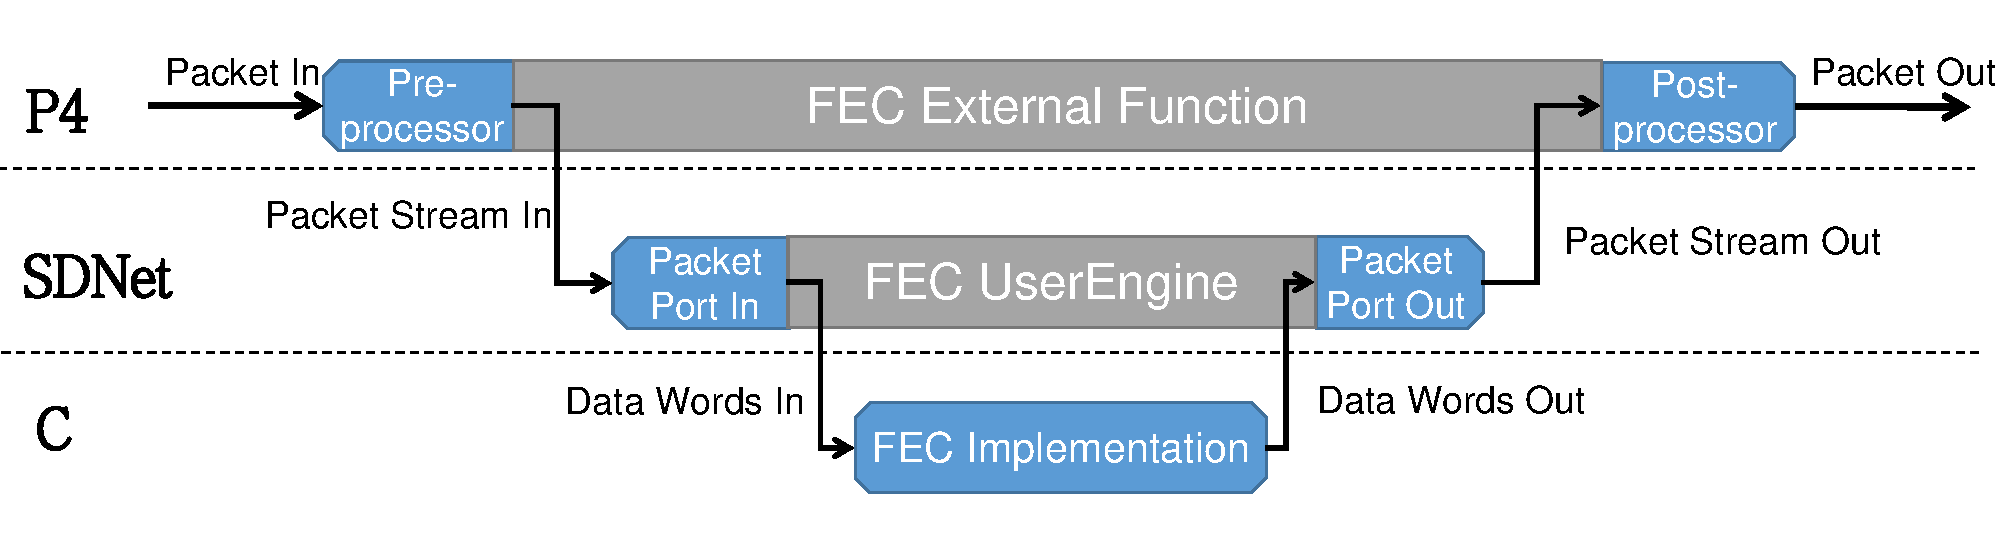
\includegraphics[width=0.4\paperwidth]{figures/sdnet-interface.pdf}
  \caption{\label{fig:sdnet-interface}Abstraction provided by each layer; grey blocks are translated to the pipeline illustrated in next level.}
\end{figure}

\iffalse
1. Both P4 and SDNet encourage programs working like a flow - you should never go back and touch anything
a second time. This ensures the efficiency of the program but also makes it harder to express complex
logics. We think it can be a future work to translate a loosely written program into one with such constrains.
Currently we do this manually by keeping in mind a dependency graph of program lines and doing a topological sort
to decide the final order. Using compound operations like
$read\_and\_add\_one$ also helps mitigating this problem.
\amd{I am not following this...and I doubt a reader with no knowledge of
  FPGAs or SDNet will be able to follow either.  What does ``go back'' mean
  in this context? What are you ordering? How is the read-and-add-one
  addressing the problem?}

2. P4 is designed particularly for header processing. There are many
irrelevant \amd{irrelevant is probably not the right word here} things not supported but
necessary in our work, especially payload processing. Most bookkeeping operations can be finished with the
help of external functions like $read\_and\_add\_one$, later implemented in C or Verilog. We also integrate the encoder
into the design by defining an external function for it. However, encoding payload through this interface can be a
great waste for both time and space due to P4's nature of passing and processing a packet as a whole, no matter how long it is. Fortunately, the
flexibility we seek can be found by redirecting SDNet's internal packet flow, which works similar to a 64-bit AXI Stream bus,
to the engine for encoder. This involves modification of less than 10 lines of code per SDNet program, and can be finished by a simple script.
\amd{...don't think this works for a reader either...  Yes, we want to make
the case that P4 doesn't allow payload processing (I suggest adding a note
about that above).  Do we want to dig into the fact that P4 doesn't give us
the expressiveness to stream payload processing, but SDNet does?  ... if
so, we'll need to setup the problem better here and be clearer about the
shape of the solution.}
\fi

\subsection{FEC Encoder}
\label{sec:impl:fec-encoder}

In this section we describe our generation of parity frames. Currently
we can only decode on a CPU; our FPGA implementation of the decode is
work-in-progress.

%The current implementation is limited to packet encoding, but our intention is
%to implement the decoder too.

In \OurSys, error correction is performed with a Reed-Solomon erasure (RSE) code~\cite{rse}.
%\hg{Note that this reference covers only error correction, not dealing with erasures}.
% Erasure codes
%require prior knowledge of which packets data is missing, as opposed to regular
%error correction codes.  This comes with the benefit of requiring fewer error
%correction bits.  RSE is a linear code, which means that every codeword can be
%obtained by a linear combination of codewords. 
Assuming we have a vector $x$,
which contains a message with $k$ symbols of $m$ bits, encoding consists merely
of multiplying $x$ with a $k \times n$ generator matrix $G$. The result is an
$n$-symbol codeword $c = xG$, where $n$ satisfies $n = k + h$.   The coefficients of the
generator matrix are constants that are determined by the values of $k$ and
$h$.
%\FIXME{Can this be cast more directly in language that corresponds to concepts used up to now
%-- packets in particular, or translate ``vector''/``message''/``symbols'' to objects that have been previously described?}
%   HG: No.  Vectors and messages are orthogonal to packets.  We could call symbols
%       bytes if we ignore $m$ as a variable, but describing an instance of the algorithm
%       as "the RSE algorithm" just to save a couple of words seems a bit ugly.
What makes RSE complex is that arithmetic operations are performed in a finite (Galois)
field to ensure that mathematical operations on integers in a finite range yield
again integers in the same range.
%\hg{I put this line back in because otherwise
%the mention of the Galois field in the resource requirements comes out of nowhere.
%If space is an issue, we can not mention this and compute resource requirements in
%units of multiplications.}
In \S\ref{sec:design}, we used $k$ and $h$ also to count packets.  This choice was intentional as
Figure~\ref{fig:Striping} demonstrates.
%\lei{I can't see the intention......}
Due to space limitations, we will not discuss RSE in more detail.
%\amd{somewhere we should be clear x is striped across corresponding bytes
%  in k packets}

\begin{figure}
  \centering
  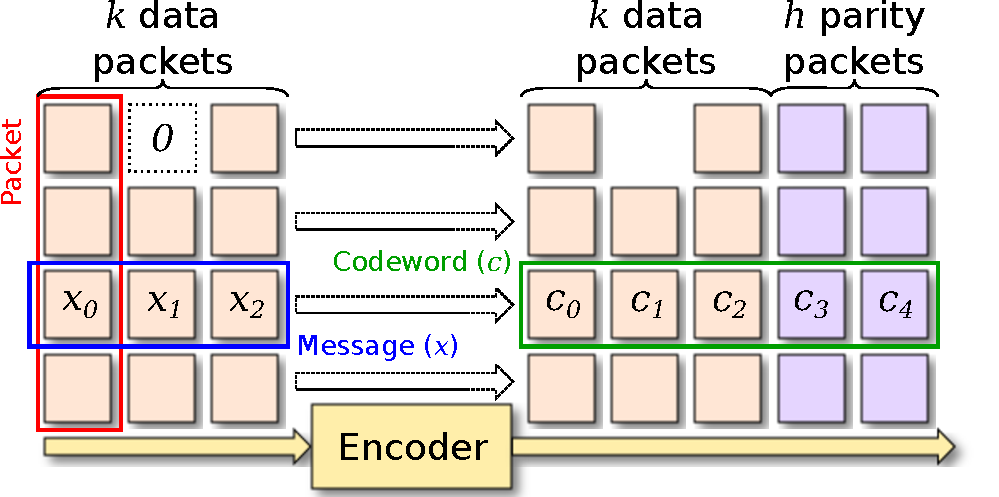
\includegraphics[width=0.4\paperwidth]{Striping.pdf}
  \caption{\label{fig:Striping} Correspondence between packet data, messages and codewords.
  }
\end{figure}

%In our encoder, the message consists of all symbols in a block that are at a
%certain offset from the start of a data packet.
%Similarly, a codeword contains
%one symbol for each output packet.  We iterate over the offset to generate
%all packets in the block.  If the packet lengths in a group differ, all packets
%will be padded up to the length of the longest packet.
%With the described data assignment, output symbols at
%different offsets are independent, so they can be computed in parallel.  The
%Ethernet MAC produces 64-bit words at a 156.25 Mhz line rate.
%For 8-bit symbols -- corresponding to bytes -- 8 matrix-vector multiplier instances running at
%line rate would suffice to sustain the throughput of the Ethernet MAC.
The encoder could be implemented to work in two ways:
non-incrementally on a block of packets, or incrementally as each
packet arrives. The non-incremental approach is more straightforward,
but incurs high latency and storage requirements, since  encoding
cannot start until all packets in a block have been received.

We opted for the incremental approach, which exploits the associativity of addition to
rearrange the terms of the sums that form the matrix-vector multiplication.
When a new input symbol is received, the partial sums for that symbol are
calculated and the output symbols are updated.

We now derive the resource requirements in terms of multiplications.
The matrix-vector multiplication requires $k \times n$
multiplications. %\FIXME{Not clear what $n$ is}
%\amd{n=k+h ?}
The first $k$ columns are an identity matrix because RSE does not alter data
packets.  The output values can be computed without multiplications.  The
remaining $kh$ multiplications are performed once for each $k$-symbol message,
resulting in $h$ multiplications per input symbol.  As a consequence, we expect that
providing a higher level of protection against erasures for a given throughput
constraint requires more hardware.  The encoder receives
packets from a 10-Gbps Ethernet MAC via a 64-bit AXI bus at a 156.25 Mhz line
rate.  For 8-bit symbols, 8 matrix-vector multiplier instances running at
line rate would suffice to sustain 10 Gbps, so altogether $8h$ Galois-field multiplications
are needed.  To save resources, we use an implementation that computes the
multiplication $m$ of $a$ and $b$ with the formula $m = e^{\log a + \log b}$.
The logarithms and exponents can be looked up in 8-bit tables with 256
entries.
%\amd{8-bit comes out of nowhere.  Do we need to state that we are working
%  with 8-bit symbols (GF(256)?) first for this to make sense?}
Such tables can be implemented in the local memories (BRAMs) of the FPGA.  
The coefficients of the generator matrix are constants.  The associated
logarithms can be precomputed, leaving only 2 lookup tables per multiplier,
resulting in a grand total of $16h$ BRAMs.

Listing~\ref{Multiplier} shows the source code of the
matrix-vector multiplier. %\FIXME{This paragraph+snippet is tricky, since we earlier dismissed using the non-incremental approach.}
It can be compiled with a regular software
compiler and executed on a microprocessor
%, for instance, 
for a software implementation or to debug the code.
In addition, Vivado HLS can generate an FPGA implementation
from the code, guided by the pragmas, which are ignored by software compilers.
A similar implementation in Verilog or VHDL requires on the order of hundreds
of lines.  The {\tt pipeline} pragma directs the tool to construct a
hardware pipeline that can start executing one invocation of the function
every clock cycle.  Vivado automatically inserts a suitable number of registers
to achieve the desired clock period.  The {\tt Par} and {\tt Gen} arrays are mapped
on BRAMs by default.  The pipeline would need {\tt MAX\_H} values from each
array per clock cycle although a dual-port BRAM can supply only 2 values.
A solution is to divide the data over multiple BRAMs that can be
accessed simultaneously.  We accomplish that for {\tt Gen} with the {\tt ARRAY\_PARTITION}
pragma.  To {\tt Par}, we applied the {\tt ARRAY\_RESHAPE} pragma to combine
all array elements into a single wide word.
%\lei{\#Shrink Candidate\#}

\begin{lstlisting}[language=C,basicstyle=\footnotesize,numbers=left,
                   captionpos=b,caption={Matrix-Vector Multiplier},
                   label=Multiplier]
void Enc(char Dat, char Par[MAX_H], int Pkt, int h) {
#pragma HLS ARRAY_RESHAPE variable=Par complete
  static char Gen[MAX_H][MAX_K] = { ... };
#pragma HLS ARRAY_PARTITION variable=Gen complete dim=0
#pragma HLS pipeline
  for (int i = 0; i < MAX_H; i++)
    Par[i] = i >= h ? Par[i] :
        GF_add(Par[i], GF_mul(Dat, Gen[i][Pkt]));
}
\end{lstlisting}

% \amd{what do we want to highlight here?
%   (1) data parallel nature of way FEC RSE is defined ... allows operate on
%   the 8 bytes in the 64b per cycle payload independently in data-parallel
%   fashion.
%   (2) as k scales up, demands more compute...which can address with more
%   hardware.
%   (3) result is can build hardware to process in a spatial pipeline at the
%   160\,MHz data rate necessary to meet 10Gbps link.
%   (4) maybe sketch out how much hardware is needed (8$\times$(2+1)$\times$k
%   BRAMs)
% }
% \hg{Ad. 2: I would say h scales up, not k, at least for the encoder.  Are you
% referring to the decoder by any chance?} \amd{yes, I got h and k confused here}

\begin{comment}
Introduce P4.
- Advantages of writing in high-level languages.
- Responsibilities of P4.
- Communication between P4 and encoder
Implementation process
- SDNet
- Vivado HLS
- Vivado
Introduce FPGA.
Top-level design
Matrix multiplication
\end{comment}

